%\newpage
\subsection*{Statement of authorship}
\renewcommand{\arraystretch}{1.5}
\begin{tabular}{m{0.25\textwidth} m{0.67\textwidth}}
    \hline \hline Paper title & Simplified equations for the magnetic field due to an arbitrarily-shaped polyhedral permanent magnet \\ \hline
    Publication status & Published \\ \hline
    Publication details & J. L. G. O’Connell, W. S. P. Robertson, and B. S. Cazzolato, ``Simplified equations for the magnetic field due to an arbitrarily-shaped polyhedral permanent magnet,'' Journal of Magnetism and Magnetic Materials, vol. 510, Sep. 2020, doi: 10.1016/j.jmmm.2020.166894. \\ \hline \hline
\end{tabular}

\vfill

\subsection*{Principal author}
\begin{tabular}{p{0.25\textwidth} m{0.67\textwidth}}
    \hline \hline Name & James O'Connell \\ \hline
    Contribution & \begin{itemize}
        \setlength\itemsep{-2mm}
        \item[-] Idea conceptualisation
        \item[-] Review of relevant literature
        \item[-] Developed polyhedral decomposition methodology
        \item[-] Performed all mathematical analysis, including computer-aided algebra and simplification of long and complication mathematical expressions
        \item[-] Identified singularities in the solutions for the field equations and treated these singularities, giving alternate formulations at the singular points
        \item[-] Implemented the algorithms in MATLAB code, including testing, analysis, and code optimisation
        \item[-] Created and executed finite element simulations to validate the mathematical algorithms and code implementation
        \item[-] Performed analysis of a polyhedral approximation of a cylindrical magnet
        \item[-] Wrote manuscript draft and created all figures
        \item[-] Finalisation of article
        \item[-] Preparation and submission for publication, including author correspondence
    \end{itemize} \\ \hline
    Percentage & 90\% \\ \hline
    Certification & This paper reports on original research conducted by the author during the period of Higher Degree by Research candidature and is not subject to any obligations or contractual agreements with a third party that would constrain its inclusion in this thesis. The author listed above is the primary author of this paper. \\ \hline
    Signature & \begin{tabular}{m{45mm} m{10mm} m{20mm}}
    \vspace{0.5mm}\includegraphics[width=0.3\textwidth]{jamesSignature.PNG} & Date: & 8 Dec 2021
    \end{tabular}
\end{tabular}

\vfill
    
\subsection*{Co-author contributions}
By signing this statement of authorship, each author certifies that:
\begin{enumerate}
    \item the candidate's stated contribution to the publication is accurate (as detailed above);
    \item permission is granted for the candidate to include the publication in the thesis; and
    \item the sum of all co-author contributions is equal to 100\% less the candidate's stated contribution.
\end{enumerate}
\begin{tabular}{m{0.25\textwidth} m{0.67\textwidth}}
    \hline \hline Name & Will Robertson \\ \hline
    Contribution & 5\% \\ \hline
    Signature & \vspace{2mm}\includegraphics[height=10mm]{willSig} \\  \hline
    Date & 16 Dec 2021 \\
    \hline \hline Name & Ben Cazzolato \\ \hline
    Contribution & 5\% \\ \hline
    Signature & \vspace{2mm} \includegraphics[height=10mm]{benSig} \\ \hline
    Date & 16 Dec 2021 \\
    \hline \hline \vfill
\end{tabular}
\renewcommand{\arraystretch}{1}
\newpage
%
\section*{\LARGE Simplified equations for the magnetic field due to an arbitrarily-shaped polyhedral permanent magnet}
James L.G. O'Connell, William S.P. Robertson, and Benjamin S. Cazzolato
\section*{Abstract}\addcontentsline{toc}{section}{\protect\numberline{}Abstract}\label{sec:p2abstract}
Due to their wide use in industrial and commercial devices, it is important to accurately and effectively model permanent magnets, leading to better magnet designs and more desirable magnetic characteristics. In recent decades, researchers have derived equations describing magnetic fields, forces, and torques, but these are usually limited to cuboid or ring-shaped magnets. Some authors have derived magnetic field equations for polyhedral magnets, allowing more general magnet shapes, but these are either not fully simplified or computationally inefficient. This paper presents a new set of simplified and exact equations describing the magnetic field produced by an arbitrarily-shaped polyhedral permanent magnet with constant uniform magnetisation and a relative permeability of unity. These equations were implemented in Matlab code and validated using finite element simulations and literature. These equations are significantly faster than finite element simulations, and can therefore be used for efficient optimisation of magnet geometry or topology, real-time simulations, and for approximation of curved surfaces of permanent magnets.
\section{Introduction}\label{sec:p2introduction}
Permanent magnets are used in a wide variety of applications, from microphones and loudspeakers to energy harvesting devices \cite{Coey2002}. They are an essential component of many electromechanical systems and are seeing widespread use with the current trend toward electric vehicles. In 2014, permanent magnets had an annual market of \$7bn USD, with hundreds of thousands of tons of neodymium magnets being manufactured annually \cite{Coey2014}. Permanent magnets see wide use in society, and it is therefore important to understand and model them effectively.

With the development of stronger magnetic materials in the late twentieth century, mathematical modelling of permanent magnets has become more common. Magnetic modelling has a high dependence on geometry, and as such, most research in this area has been undertaken on simple geometries such as cuboidal and ring-shaped permanent magnets.

Cuboid magnets are extremely prevalent in society and industry, and have therefore received considerable attention in literature. Additionally, their geometry is simple, leading to simple field equations. In 1984, \textcite{Akoun1984} published the magnetic field equations for a vertically-magnetised cuboid magnet by considering a magnetic charge distribution over the surface of the magnet. \textcite{Bancel1999} suggested that the magnetic field produced by a cuboid can be thought of as field contributions from each of the eight vertices, or `nodes'. Several decades later, \textcite{Ravaud2009} extended these equations to include an arbitrary magnetisation direction by using superposition of mutually perpendicular magnetisations. However, these equations do not consider mathematical singularities, which often exist at points inline with a magnet edge. Other authors have gone beyond field calculations by publishing equations describing forces and torques between parallel cuboid magnets with parallel magnetisations \cite{Akoun1984,Allag2009}, parallel cuboid magnets with arbitrary magnetisations \cite{Janssen2011}, and rotated cuboid magnets \cite{Dam2016}. However, all aforementioned equations are limited to cuboid magnets, and are invalid for other magnet geometries.

Like cuboid magnets, cylindrical and ring-shaped magnets have seen wide use in industry, and have also received considerable attention in literature. They exhibit simple geometry in a cylindrical coordinate system, leading to relatively simple field equations. In 1995, \textcite{Furlani1995} derived the magnetic field due to radially-magnetised ring sectors, but these equations are not fully analytic and require some numerical integration. Ravaud et al.\ \cite{Ravaud2008a,Ravaud2010} improved these equations by using elliptic integrals, leading to fewer numeric integrals. In another study, \textcite{Ravaud2008} considered the simpler geometry of a full ring magnet rather than a sector. With this assumption, they found expressions for the magnetic field produced by both radially- and axially-magnetised ring magnets using elliptic integrals. More recently, \textcite{Caciagli2018} derived simpler equations describing the magnetic field produced by cylindrical magnets. However, these equations are again limited to a specific geometry and other geometries require separate solutions.

Although cuboidal and ring magnets have been studied extensively, few other geometries have received attention. Papers by \textcite{Janssen2009,Janssen2010a}, \textcite{Compter2010}, \textcite{Rubeck2013}, and \textcite{OConnell2020} presented analytic equations for the magnetic field due to a general polyhedral permanent magnet with constant uniform magnetisation and unity relative permeability. These equations can be used for any magnet composed of flat faces, and can also be used to approximate curved surfaces, allowing approximate solutions of any magnet geometry. However, the studies by \textcite{Janssen2009,Janssen2010a} and \textcite{Compter2010} present equations which are not fully simplified, limiting their computational efficiency. The equations presented by \textcite{Rubeck2013} and \textcite{OConnell2020} are simpler, but inefficient for a large number of field evaluations because they require processing of the geometry for every field point. Furthermore, these studies do not consider mathematical singularities, which cause the magnetic field evaluations to become undefined at some locations.

This paper attempts to alleviate both of these issues by presenting new magnetic field equations for a general polyhedral permanent magnet which are fully simplified, computationally efficient, and include singularity treatment. These field equations are derived by the authors in Section \ref{sec:p2methodology} and validated using both past literature and finite element simulations in Section \ref{sec:p2validation} before the paper is concluded in Section \ref{sec:p2conclusion}.
\section{Methodology}\label{sec:p2methodology}
A permanent magnet with magnetisation vector \(\mathbf{M}\) can be modelled as a collection of magnetic charges described by the magnetic charge model \cite{Furlani2001}. The magnetic field \(\mathbf{B}\) at a point in space outside the magnet \(\mathbf{x}\) can be calculated using the charge model given by

\begin{equation}
\label{eqn:p2chargemodel}
\mathbf{B}\left( \mathbf{x} \right) = \frac{\mu_0}{4\pi} \left( \oint_{S} \left( \mathbf{M} \cdot \hat{\mathbf{n}} \right) \frac{\mathbf{x} - \mathbf{x}'}{\left| \mathbf{x} - \mathbf{x}' \right|^3} \ ds' - \int_{V} \left( \nabla \cdot \mathbf{M} \right) \frac{\mathbf{x} - \mathbf{x}'}{\left| \mathbf{x} - \mathbf{x}' \right|^3} \ dv' \right) \text{,}
\end{equation}

\noindent where \(\mu_0\) is the permeability of free space, \(V\) is the magnet volume, \(S\) is the magnet surface, \(\mathbf{x}'\) is a point in or on the magnet, and \(\hat{\mathbf{n}} = \left[ n_x, n_y, n_z \right]\) is the outward-facing unit normal vector of the magnet surface. If the magnet is assumed ideal; that is, the magnetisation \(\mathbf{M}\) is assumed uniform and constant and the relative permeability is assumed unity, the volume integral disappears as \(\nabla \cdot \mathbf{M} = 0\), leaving only the surface integral

\begin{equation}
\label{eqn:p2chargeB}
\mathbf{B}\left( \mathbf{x} \right) = \frac{\mu_0}{4\pi} \oint_{S} \left( \mathbf{M} \cdot \hat{\mathbf{n}} \right) \frac{\mathbf{x} - \mathbf{x}'}{\left| \mathbf{x} - \mathbf{x}' \right|^3} \ ds' \text{.}
\end{equation}

\noindent Equation (\ref{eqn:p2chargeB}) implies the magnet can be considered a set of \(n\) magnetically charged surfaces \(S_{\!i}\), with the total field given by

\begin{equation}
\label{eqn:p2chargeBdiscrete}
\mathbf{B}\left( \mathbf{x} \right) = \sum_{i=1}^n \frac{\mu_0}{4\pi} \int_{S_i} \left( \mathbf{M} \cdot \hat{\mathbf{n}}_i \right) \frac{\mathbf{x} - \mathbf{x}'}{\left| \mathbf{x} - \mathbf{x}' \right|^3} \ ds_i' = \sum_{i=1}^n \textbf{B}_i\left(\textbf{x}\right) \text{,}
\end{equation}

\noindent where \(\textbf{B}_i\left(\mathbf{x}\right)\) is the magnetic field contribution of the surface \(S_{\!i}\).

The total magnetic field due to the magnet can be found by solving Equation (\ref{eqn:p2chargeBdiscrete}), i.e., summing the field contributions from each surface \(S_{\!i}\) to give the total magnetic field. To do this, first the polyhedral magnet must be decomposed into a set of charged surfaces, as described in the following section.

\subsection{Polyhedral decomposition}\label{sec:p2polyhedrondecomposition}

To calculate the magnetic field at a point \(\mathbf{x} = \left[ x, y, z\right]\) due to a polyhedral permanent magnet with surface \(S\), the magnet is considered a collection of polygonal surfaces \(S_{\!i}\). The field calculation begins by considering one polygonal surface \(S_{\!i}\) with magnetic charge density \(\mathbf{M} \cdot \hat{\mathbf{n}}_i\), where \(\hat{\mathbf{n}}_i\) is the outward-facing unit normal vector of the surface \(S_{\!i}\). This surface and the point \(\mathbf{x}\) are rotated in 3D space about the origin such that \(S_{\!i}\) is parallel to the \(XY\)-plane; that is, \(S_{\!i}\) is rotated such that its normal vector is parallel to the \(z\)-axis. This is done by postmultiplying \(\mathbf{x}\) and each vertex of \(S_{\!i}\) by the rotation matrix \(R\), given by

\begin{equation}
R = \begin{bmatrix}
m & 0 & n_x \\[4pt]
-n_xn_y/m & n_z/m & n_y \\[4pt]
-n_xn_z/m & -n_y/m & n_z
\end{bmatrix} \text{,}
\end{equation}

\noindent where \(m = \sqrt{n_y^2+n_z^2}\). A full derivation of \(R\) is given in \ref{sec:p2Rderivation}. Note that if \(\hat{\mathbf{n}}_i = \left[\pm1,0,0\right]\), then the surface is parallel to the \(YZ\) plane and \(n_y = n_z = 0 \implies m = 0\) and \(R\) is undefined. In this case, the limit as \(n_z\) approaches 0 from the positive side is taken and \(R\) should instead be defined as

\begin{equation}
R = \begin{bmatrix}
\phantom{-}0 & 0 & 1 \\
\phantom{-}0 & 1 & 0 \\
-1 & 0 & 0 \end{bmatrix} \text{.}
\end{equation}

After rotation, the point at which the field is to be computed is given by \(\mathbf{x}_r = \mathbf{x}R\) and the surface \(S_{\!i}\) is parallel to the \(XY\)-plane. Lines are drawn through each vertex of the polygonal surface parallel to the \(y\)-axis, dividing the polygon into a series of trapezia \(T_{\!j}\), as shown in Figure \ref{fig:p2polyhedrondecomposition}. Note that for this work, a triangle is considered a degenerate case of a trapezium with one of the parallel sides having a length of zero. The magnetic field contribution of each trapezium is computed using the solution to Equation (\ref{eqn:p2chargeB}) described in Section \ref{sec:p2fieldcalc}.
\begin{figure}[h]
	\centering
	\begin{subfigure}{0.6\textwidth}
	\centering
	\begin{tikzpicture}[scale=2.5]
		\coordinate(c1) at (-0.47943,0.87758);
		\coordinate(c2) at (-0.98278,-0.18477);
		\coordinate(c3) at (-0.12797,-0.99178);
		\coordinate(c4) at (0.90369,-0.42818);
		\coordinate(c5) at (0.68648,0.72715);
	\draw (c1) -- (c2) -- (c3) -- (c4) -- (c5) -- cycle;
		\draw[->] (-1.2,-1.3) -- (-0.2,-1.3);
		\draw[->] (-1.2,-1.3) -- (-1.2,-0.3);		\node(x) at (-0.1,-1.3) {\(x\)};
		\node(y) at (-1.2,-0.2) {\(y\)};
		
		\node(Si) at (0,0) {\(S_i\)};
	\end{tikzpicture}
	\caption{}\label{fig:p2polyhedrondecompositiona}
\end{subfigure}

\vspace{40pt}

\begin{subfigure}{0.6\textwidth}
	\centering
	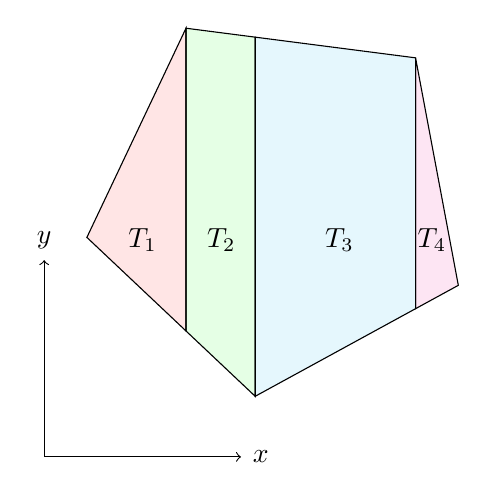
\begin{tikzpicture}[scale=2.5]
		\coordinate(c1) at (-0.98278,-0.18477);
		\coordinate(c2) at (-0.98278,-0.18477);
		\coordinate(c3) at (-0.47943,0.87758);
		\coordinate(c4) at (-0.47943,-0.65998);
		\filldraw[fill=red, fill opacity=0.1] (c1) -- (c2) -- (c3) -- (c4) -- cycle;
		\coordinate(c5) at (-0.47943,-0.65998);
		\coordinate(c6) at (-0.47943,0.87758);
		\coordinate(c7) at (-0.12797,0.83224);
		\coordinate(c8) at (-0.12797,-0.99178);
		\filldraw[fill=green, fill opacity=0.1] (c5) -- (c6) -- (c7) -- (c8) -- cycle;
		\coordinate(c9) at (-0.12797,-0.99178);
		\coordinate(c10) at (-0.12797,0.83224);
		\coordinate(c11) at (0.68648,0.72715);
		\coordinate(c12) at (0.68648,-0.54684);
		\filldraw[fill=cyan, fill opacity=0.1] (c9) -- (c10) -- (c11) -- (c12) -- cycle;
		\coordinate(c13) at (0.68648,-0.54684);
		\coordinate(c14) at (0.68648,0.72715);
		\coordinate(c15) at (0.90369,-0.42818);
		\coordinate(c16) at (0.90369,-0.42818);
		\filldraw[fill=magenta, fill opacity=0.1] (c13) -- (c14) -- (c15) -- (c16) -- cycle;
		\draw[->] (-1.2,-1.3) -- (-0.2,-1.3);
		\draw[->] (-1.2,-1.3) -- (-1.2,-0.3);		\node(x) at (-0.1,-1.3) {\(x\)};
		\node(y) at (-1.2,-0.2) {\(y\)};
		
		% Label trapezia
		\node(t1) at (-0.7,-0.2) {\(T_1\)};
		\node(t2) at (-0.3,-0.2) {\(T_2\)};
		\node(t3) at (0.3,-0.2) {\(T_3\)};
		\node(t4) at (0.77,-0.2) {\(T_4\)};
	\end{tikzpicture}
	\caption{}\label{fig:p2polyhedrondecompositionb}
\end{subfigure}

	\caption{After the polygonal surface \(S_{\!i}\) has been rotated such that it is parallel to the \(XY\)-plane (\subref{fig:p2polyhedrondecompositiona}), lines are drawn through each vertex parallel to the \(y\)-axis, dividing the polygon into trapezia (\subref{fig:p2polyhedrondecompositionb}).}
	\label{fig:p2polyhedrondecomposition}
\end{figure}

\subsection{Magnetic field calculation of charged trapezia}\label{sec:p2fieldcalc}

\begin{figure}
	\centering
	\def\lim{10}

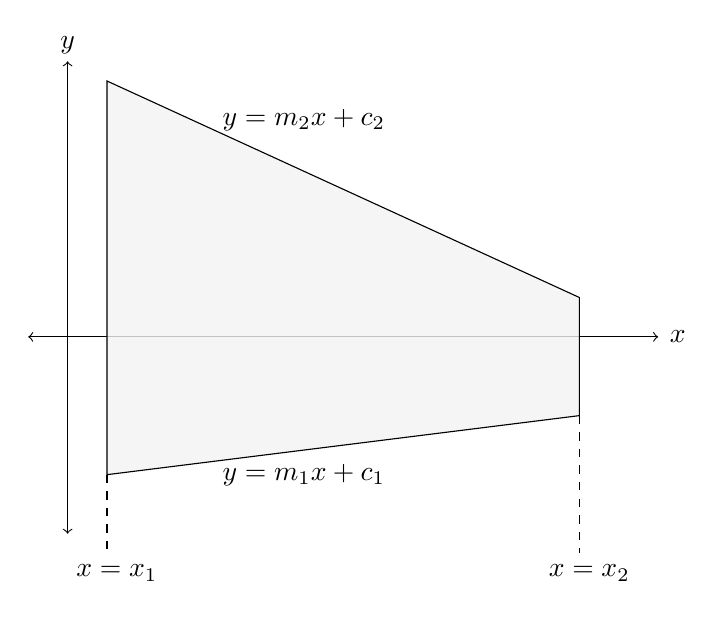
\begin{tikzpicture}[scale=0.5]
	\coordinate(negx) at (-1,0);
	\coordinate(posx) at (\lim+2,0);
	\coordinate(negy) at (0,-5);
	\coordinate(posy) at (0,7);
	
	\coordinate(TL) at (1,6.5);
	\coordinate(BL) at (1,-3.5);
	\coordinate(TR) at (\lim,1);
	\coordinate(BR) at (\lim,-2);
	
	\draw[<->] (negx) -- (posx);
	\draw[<->] (negy) -- (posy);
	\filldraw[fill=black!5, fill opacity=0.8] (BL) -- (BR) -- (TR) -- (TL) -- cycle;
	
	\draw[dashed] (BL) -- (1,-5.5);
	\node(x1) at (1.25,-6) {\(x = x_1\)};
	\draw[dashed] (BR) -- (\lim,-5.5);
	\node(x2) at (\lim+0.25,-6) {\(x = x_2\)};
	\node(m1c1) at (6,-3.5) {\(y=m_1x+c_1\)};
	\node(m2c2) at (6,5.5) {\(y=m_2x+c_2\)};
	\node(x) at (\lim+2.5,0) {\(x\)};
	\node(y) at (0,7.4) {\(y\)};
\end{tikzpicture}
	\caption{A magnetically charged trapezial surface. It is parallel to the \(XY\)-plane with \(z\)-coordinate \(z = z'\) and a pair of opposite edges parallel to the \(y\)-axis.}
	\label{fig:p2trapezium}
\end{figure}

Given a magnetically charged trapezium parallel to the \(XY\)-plane at \(z = z'\), with the parallel lines having equations \(x = x_1\) and \(x = x_2\) and the non-parallel lines having equations \mbox{\(y = m_1x+c_1\)} and \mbox{\(y = m_2x+c_2\)} (shown in Figure \ref{fig:p2trapezium}), the magnetic field contribution \(\left[B_{xj},B_{yj},B_{zj}\right]\) at a point \(\mathbf{x}_r = \left[ x_r, y_r, z_r \right]\) is given by

\begin{equation}
	\label{eqn:p2myintegral}
	\left[ B_{xj}, B_{yj}, B_{zj} \right] = \frac{\mu_0}{4\pi} \int_{x_1}^{x_2} \int_{m_1x'+c_1}^{m_2x'+c_2} \left( \mathbf{M} \cdot \hat{\mathbf{n}} \right) \left[ I_x, I_y, I_z \right] \ dy' \ dx'
\end{equation}

\noindent where

\begin{align}
	I_x &= \frac{\left[x_r-x'\right]}{\left(\left(x_r-x'\right)^2+\left(y_r-y'\right)^2+\left(z_r-z'\right)^2\right)^{3/2}} \text{,} \nonumber \\
	I_y &=  \frac{\left[y_r-y'\right]}{\left(\left(x_r-x'\right)^2+\left(y_r-y'\right)^2+\left(z_r-z'\right)^2\right)^{3/2}} \text{,} \\
	I_z &=  \frac{\left[z_r-z'\right]}{\left(\left(x_r-x'\right)^2+\left(y_r-y'\right)^2+\left(z_r-z'\right)^2\right)^{3/2}} \text{.} \nonumber
\end{align}

After solving this difficult integral and simplifying the result\footnote{The full derivation for this solution is outlined in Appendix \ref{app:fieldEquations}}, the authors derived the following solution to Equation (\ref{eqn:p2myintegral}).

\begin{align}\label{eqn:p2fieldequation}
\begin{split}
B_{xj} &= \frac{\mu_0}{4\pi} \left(\mathbf{M} \cdot \hat{\mathbf{n}}\right) \sum_{p=1}^2 \sum_{q=1}^2 \left[ \left( -1 \right) ^{p+q} \left( \ln \left( T_{pq} \right) - \frac{m_p}{\sqrt{1+m_p^2}} \ln \left(S_{\!pq}\right) \right) \right] \\
B_{yj} &= \frac{\mu_0}{4\pi} \left(\mathbf{M} \cdot \hat{\mathbf{n}}\right) \sum_{p=1}^2 \sum_{q=1}^2 \left[ \left( -1 \right)^{p+q} \frac{1}{\sqrt{1+m_p^2}} \ln \left( S_{\!pq} \right) \right] \\
B_{zj} &= \frac{\mu_0}{4\pi} \left(\mathbf{M} \cdot \hat{\mathbf{n}}\right) \sum_{p=1}^2 \sum_{q=1}^2 \Bigg[ \left( -1 \right) ^{p+q} \arctan \left( U_{pq} \right) \Bigg] \text{,}
\end{split}
\end{align}

\noindent with

\begin{align}\label{eqn:p2intermediatevars}
\begin{split}
X &= x_q - x_r \\
Y &= c_p + m_px_q - y_r \\
Z &= z' - z_r \\
R_{pq} &= \sqrt{X^2 + Y^2 + Z^2} \\
S_{\!pq} &= X + m_pY + \sqrt{1+m_p^2}R_{pq} \\
T_{pq} &= R_{pq} + Y \\
U_{pq} &= \frac{m_p\left(X^2+Z^2\right)-XY}{ZR_{pq}} \text{.}
\end{split}
\end{align}

Equation (\ref{eqn:p2fieldequation}) describes the magnetic field produced by the magnetically charged trapezium shown in Figure \ref{fig:p2trapezium}. Further processing is required to calculate the magnetic field produced by a polyhedral magnet, as described in the following sections.

\subsubsection{Special case when \(m_p = 0\)}

Equation (\ref{eqn:p2fieldequation}) can be applied to a cuboidal magnet by using six rectangular faces with \(m_p = 0\) for all \(p\). Substituting \(m_p = 0\) into Equations (\ref{eqn:p2fieldequation}) and (\ref{eqn:p2intermediatevars}) gives the following simplified equations for a cuboidal magnet.

\begin{align}\label{eqn:p2cuboidequation}
\begin{split}
B_x &= \frac{\mu_0}{4\pi} \left(\mathbf{M} \cdot \hat{\mathbf{n}}\right) \sum_{p=1}^2 \sum_{q=1}^2 \left[ \left( -1 \right) ^{p+q} \ln \left( T_{pq} \right) \right] \\
B_y &= \frac{\mu_0}{4\pi} \left(\mathbf{M} \cdot \hat{\mathbf{n}}\right) \sum_{p=1}^2 \sum_{q=1}^2 \left[ \left( -1 \right) ^{p+q} \ln \left( S_{\!pq} \right) \right] \\
B_z &= \frac{\mu_0}{4\pi} \left(\mathbf{M} \cdot \hat{\mathbf{n}}\right) \sum_{p=1}^2 \sum_{q=1}^2 \left[ \left( -1 \right) ^{p+q} \arctan \left( U_{pq} \right) \right] \text{,}
\end{split}
\end{align}

\noindent with

\begin{align}\label{eqn:p2cuboidvars}
\begin{split}
X &= x_q - x_r \\
Y &= c_p - y_r \\
Z &= z' - z_r \\
R_{pq} &= \sqrt{X^2 + Y^2 + Z^2} \\
S_{\!pq} &= X + R_{pq} \\
T_{pq} &= R_{pq} + Y \\
U_{pq} &= \frac{-XY}{ZR_{pq}} \text{.}
\end{split}
\end{align}

It can be shown that these equations are equivalent to those published by \textcite{Akoun1984}, \textcite{Bancel1999}, and \textcite{Ravaud2009}, verifying Equation (\ref{eqn:p2fieldequation}) for cuboidal magnets\footnote{The equations in \cite{Akoun1984}, \cite{Bancel1999}, and \cite{Ravaud2009} are of the same form, but with different variable names.}.

\subsection{Polyhedral recomposition}

Once the magnetic field contributions from each trapezium \(T_{\!j}\) is computed, all contributions are summed to give the total field due to the polygonal surface \(S_{\!i}\),

\begin{equation}
\begin{bmatrix}
B_{xi} & B_{yi} & B_{zi}
\end{bmatrix} = \sum_j \begin{bmatrix}
B_{xj} & B_{yj} & B_{zj} \end{bmatrix} \text{.}
\end{equation}

\noindent This magnetic field vector is then postmultiplied by \(R^\text{T}\) to give the field due to \(S_{\!i}\) in the original coordinate system,

\begin{equation}
\textbf{B}_i\left(\textbf{x}\right) = \begin{bmatrix}
B_{xi} & B_{yi} & B_{zi} \end{bmatrix}
R^\textsf{T} \text{,}
\end{equation}

\noindent where \(R^{\textsf{T}}\) is the transpose of \(R\).

This process is repeated for each face of the polyhedron. Finally, the field contributions from each polygonal face \(S_{\!i}\) are summed to give the total magnetic field at the point \(\mathbf{x}\) due to the polyhedral permanent magnet,

\begin{equation}
\textbf{B}\left(\textbf{x}\right) = \sum_{i=1}^n \textbf{B}_i\left(\textbf{x}\right) \text{.}
\end{equation}

\subsection{Singularity treatment}

Singularities can be found in Equation (\ref{eqn:p2fieldequation}) when \(S_{\!pq} = 0\), when \(T_{pq} = 0\), or when \(U_{pq} = 0/0\). The regions in which each of these singularities occur are shown in Figure \ref{fig:p2singularities}. Under these conditions, the magnetic field given by Equation (\ref{eqn:p2fieldequation}) is undefined, so these singularities must be resolved to give a robust magnetic field solution.

\begin{figure}
	\centering
	\def\myscale{0.3}
\def\greythick{50}

\begin{subfigure}{0.45\textwidth}
\centering
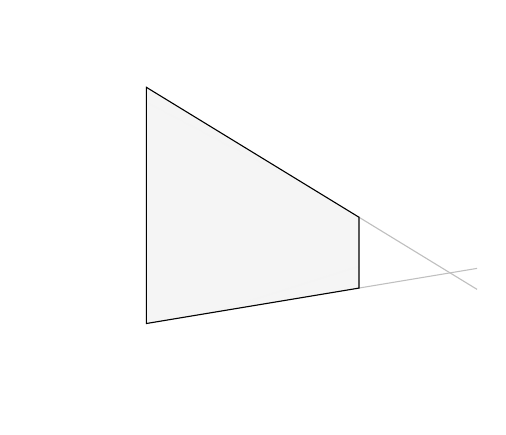
\begin{tikzpicture}[scale=\myscale]
	\coordinate(TL) at (1,6.5);
	\coordinate(BL) at (1,-3.5);
	\coordinate(TR) at (10,1);
	\coordinate(BR) at (10,-2);
	
	% Draw some white lines to make sure all figures are the same size:
	\draw[white] (-4,8.5) -- (15,-1.5);
	\draw[white] (-4,-5.5) -- (15,0.5);
	\draw[white] (1,-7) -- (1,9);
	\draw[white] (11,-7) -- (11,9);
	
	% Draw the singular regions:
	\draw[gray!\greythick] (10,1) -- (15,-2.05555556);
	\draw[gray!\greythick] (10,-2) -- (15,-1.16666667);
	
	% Draw the trapezium:
	\filldraw[fill=black!5, fill opacity=0.8] (BL) -- (BR) -- (TR) -- (TL) -- cycle;
\end{tikzpicture}
\caption{}\label{fig:p2singularitiesa}
\end{subfigure}
\begin{subfigure}{0.45\textwidth}
\centering
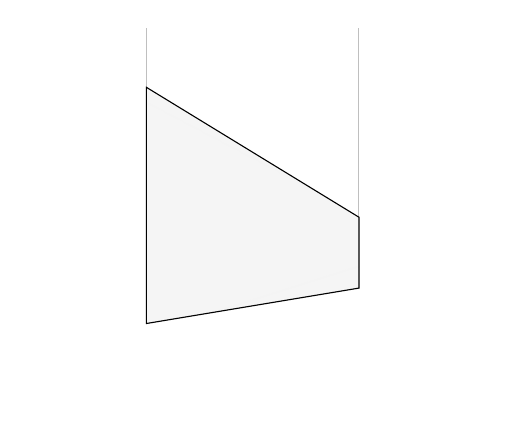
\begin{tikzpicture}[scale=\myscale]
    \coordinate(TL) at (1,6.5);
    \coordinate(BL) at (1,-3.5);
    \coordinate(TR) at (10,1);
    \coordinate(BR) at (10,-2);
	
	% Draw some white lines to make sure all figures are the same size:
	\draw[white] (-4,8.5) -- (15,-1.5);
	\draw[white] (-4,-5.5) -- (15,0.5);
	\draw[white] (1,-7) -- (1,9);
	\draw[white] (11,-7) -- (11,9);
	
	% Draw the singular regions:
	\draw[gray!\greythick] (1,6.5) -- (1,9);
	\draw[gray!\greythick] (10,1) -- (10,9);
	
	% Draw the trapezium:
	\filldraw[fill=black!5, fill opacity=0.8] (BL) -- (BR) -- (TR) -- (TL) -- cycle;
\end{tikzpicture}
\caption{}\label{fig:p2singularitiesb}
\end{subfigure}
\begin{subfigure}{0.45\textwidth}
    \centering
    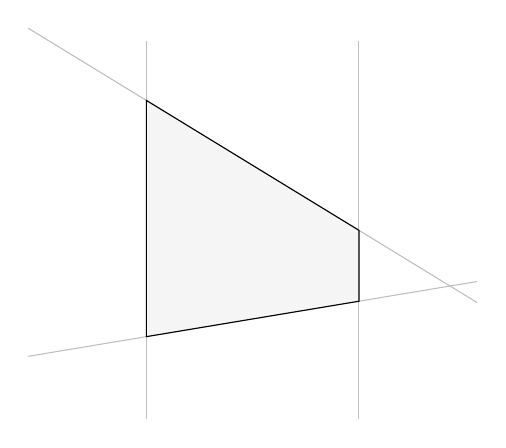
\begin{tikzpicture}[scale=\myscale]
    \coordinate(TL) at (1,6.5);
    \coordinate(BL) at (1,-3.5);
    \coordinate(TR) at (10,1);
    \coordinate(BR) at (10,-2);
	
	% Draw the singular regions:
	\draw[gray!\greythick] (-4,9.55555556) -- (15,-2.05555556);
	\draw[gray!\greythick] (-4,-4.33333333) -- (15,-1.16666667);
	\draw[gray!\greythick] (1,-7) -- (1,9);
	\draw[gray!\greythick] (10,-7) -- (10,9);
	
	% Draw the trapezium:
	\filldraw[fill=black!5, fill opacity=0.8] (BL) -- (BR) -- (TR) -- (TL) -- cycle;
\end{tikzpicture}
\caption{}\label{fig:p2singularitiesc}
\end{subfigure}


	\caption{The regions around a trapezium in which singularities occur. \(S_{\!pq} = 0\) along the grey lines in (\subref{fig:p2singularitiesa}), \(T_{pq} = 0\) along the grey lines in (\subref{fig:p2singularitiesb}), and \(U_{pq} = 0/0\) along the grey lines in (\subref{fig:p2singularitiesc}).}
	\label{fig:p2singularities}
\end{figure}

\subsubsection{Solving \(S_{\!pq} = 0\)}

Substituting \(S_{\!pq} = 0\) into Equation (\ref{eqn:p2intermediatevars}) implies that \(X < 0\), \(Y = m_pX\), and \(Z = 0\). Therefore, any point inline with one of the non-parallel edges and to the right of any trapezium, shown in Figure \ref{fig:p2singularitiesa}, will lead to a singularity in the equations. This can be solved by applying L'H\^{o}pital's rule twice, giving Equation (\ref{eqn:p2Ssingsol}).

When evaluating Equations (\ref{eqn:p2fieldequation}) and (\ref{eqn:p2intermediatevars}), if for any pair \(\left(p,q\right)\), \(X < 0\), \(Y = m_pX\), and \(Z = 0\), this singularity is solved by the redefinition

\begin{equation}\label{eqn:p2Ssingsol}
S_{\!pq} = \frac{1}{R_{pq}} \text{.}
\end{equation}

\subsubsection{Solving \(T_{pq} = 0\)}

Substituting \(T_{pq} = 0\) into Equation (\ref{eqn:p2intermediatevars}) implies that \(X = 0\), \(Y < 0\), and \(Z = 0\). Therefore, if a point is inline with one of the parallel edges of any trapezium and above it, shown in Figure \ref{fig:p2singularitiesb}, a singularity will occur. This can be solved by again applying L'H\^{o}pital's rule twice, giving Equation (\ref{eqn:p2Tsingsol}).

When evaluating Equations (\ref{eqn:p2fieldequation}) and (\ref{eqn:p2intermediatevars}), if for any pair \(\left(p,q\right)\), \(X = Z = 0\) and \(Y < 0\), this singularity is solved by the redefinition

\begin{equation}\label{eqn:p2Tsingsol}
T_{pq} = \frac{1}{R_{pq}} \text{.}
\end{equation}

\subsubsection{Solving \(U_{pq} = 0/0\)}

Setting the denominator of \(U_{pq}\) to 0 in Equation (\ref{eqn:p2intermediatevars}) gives \(Z = 0\) since \(R_{pq} > 0\) for any point not coincident with a vertex. If \(Z = 0\), then the numerator of \(U_{pq}\) also goes to 0 when either \(X = 0\) or \(Y = m_pX\). Therefore, this singularity occurs when \(Z = X = 0\), or when \(Z = Y - m_pX = 0\). The singular regions are shown in Figure \ref{fig:p2singularitiesc}.

Solving the former case, \(X = Z = 0\), requires the use of L'H\^{o}pital's rule once, giving \(U_{pq} = \sgn\left(Y\right)\). However, due to the summation over \(p\) and the term \(\left(-1\right)^{p+q}\) in Equation (\ref{eqn:p2fieldequation}), \(U_{pq}\) can simply be set to 0.

The latter case, namely, \(Z = Y - m_pX = 0\), has a more trivial solution. Since \(Y = m_pX\), the numerator simplifies to \(-m_pZ^2\), leaving \(U_{pq} = -m_pZ/R_{pq}\). Since \(Z = 0\) and \(R_{pq} > 0\), this becomes \(U_{pq} = 0\). These two results give Equation (\ref{eqn:p2Usingsol}).

When evaluating Equations (\ref{eqn:p2fieldequation}) and (\ref{eqn:p2intermediatevars}), if for any pair \(\left(p,q\right)\), \(Z = X = 0\) or \(Z = Y-mX = 0\), this singularity is solved by the redefinition

\begin{equation}\label{eqn:p2Usingsol}
U_{pq} = 0 \text{.}
\end{equation}

\subsection{Computational considerations}

In contrast with previous solutions \cite{Rubeck2013,OConnell2020}, the solution formulated in this paper has been derived to allow the computation of a matrix of points \(P\) to be evaluated with only a single polyhedral decomposition and rotation routine. If \(n\) points are defined as \(\left[x_1, y_1, z_1\right], \dotsc, \left[x_n, y_n, z_n\right]\), then \(P\) is defined by the \(\left( n \times 3\right)\) matrix

\begin{equation}
P = \begin{bmatrix}
x_1 & y_1 & z_1 \\
\vdots & \vdots & \vdots \\
x_n & y_n & z_n
\end{bmatrix} \text{.}
\end{equation}

For a given polygonal facet \(S_{\!i}\) with associated rotation matrix \(R\), \(P_r = PR\) gives a list of rotated points at which the magnetic field can be calculated. Equation (\ref{eqn:p2fieldequation}) is applied to each row of \(P_r\), and the magnetic field components rotated back to the original coordinate system after the computation of the field at all points in \(P_r\). In this way, polyhedron decomposition occurs only once, independent of the number of points, therefore reducing overhead and increasing efficiency.

Using this methodology on a polyhedron with \(E\) edges and \(F\) faces, a maximum of \(2E - F\) trapezia are required (see \ref{sec:p2numtrap}), giving an upper bound on the number of calculations required. If the magnetic field is to be evaluated at \(n\) points, then Equation (\ref{eqn:p2fieldequation}) must be computed a total of up to \(n\left(2E-F\right)\) times with up to \(2F\) total rotations. Therefore, if each computation of Equation (\ref{eqn:p2fieldequation}) takes \(t_n\) seconds and the average overhead for each calculation is \(t_o\), an upper bound for the total expected calculation time is

\begin{equation}
t_{\text{expected}} \leq \left(2E-F\right)\left(t_o + nt_n \right) \text{.}
\end{equation}

\noindent This equation shows that the calculation time scales approximately linearly with the number of points at which the field is calculated.

This methodology was implemented in vectorised Matlab code without parallelisation in Matlab R2017b (MathWorks, Inc., Natick, MA, USA). This was run on a workstation PC with an Intel Xeon E3-1240 v5 at 3.50GHz and 16GB of memory using Windows 10 Enterprise. In an effort to approximate the constants \(t_o\) and \(t_n\), a randomly generated polyhedron was defined, and the magnetic field calculated at a large number of points near the polyhedron. On this particular computer hardware, \(t_o\) was in the order of several milliseconds (\(10^{-3}\) seconds) and \(t_n\) was in the order of several hundred nanoseconds (\(10^{-7}\) seconds). These values will vary when using different computer hardware and software, but the constants stated here give an approximation of calculation time before the algorithm is executed.

This methodology excels when calculating the magnetic field at a large number of points. This is because the rotation and decomposition routines are the slowest parts of the algorithm, but only occur once, no matter the number of field calculations. The computation of Equation (\ref{eqn:p2fieldequation}) is orders of magnitude faster than the rotation and decomposition routine, and thus a larger number of field calculations has little effect on the computation time.

The Matlab implementation of the algorithm presented in this paper is available as the file polyhedronField.m at

\noindent \url{github.com/jlgO'Connell/polyhedralMagnet}.

\section{Validation}\label{sec:p2validation}
To validate this methodology, finite element simulations were performed using the Maxwell3D package from ANSYS Electronics Desktop 2018.0 (ANSYS, Inc., Berkeley, CA, USA). Two cases were considered, with the magnetic field of each being calculated analytically using the above methodology and numerically using Maxwell3D. The second case was further validated using the analytic solutions presented by \textcite{Caciagli2018}. The magnetic field for both cases was also calculated using methodology from previously published and validated work by the current authors \cite{OConnell2020}. In the subsequent sections, the results and computation time from the current methodology are compared to those of the finite element simulations, literature, and earlier work.

\subsection{Pyramid frustum magnet}

\begin{figure}
	\centering
	\def\lim{13}

\tdplotsetmaincoords{70}{45}
\begin{tikzpicture}[scale=0.13,tdplot_main_coords]

% Define coordinates:
\coordinate(ppb) at (15,15,-20);
\coordinate(pnb) at (15,-15,-20);
\coordinate(nnb) at (-15,-15,-20);
\coordinate(npb) at (-15,15,-20);
\coordinate(ppt) at (10,10,0);
\coordinate(pnt) at (10,-10,0);
\coordinate(nnt) at (-10,-10,0);
\coordinate(npt) at (-10,10,0);

% Fill in polygons:
\filldraw[fill=white] (ppt) -- (pnt) -- (nnt) -- (npt) -- cycle;
\filldraw[fill=white] (ppt) -- (ppb) -- (pnb) -- (pnt) -- cycle;
\filldraw[fill=white] (pnt) -- (nnt) -- (nnb) -- (pnb) -- cycle;

% Axes:
\draw[->] (0,0,0) -- (\lim,0,0);
\draw[->] (0,0,0) -- (0,\lim,0);
\draw[->] (0,0,0) -- (0,0,\lim);
\node(xaxis) at (\lim+2,0,0) {\(x\)};
\node(yaxis) at (0,\lim+2,0) {\(y\)};
\node(zaxis) at (0,0,\lim+2) {\(z\)};

% Dimensions:
\draw[<->] (20,-18,-20) -- (20,12,-20);
\node(botdim) at (26,-5,-20) {30mm};
\draw[<->] (-12,-20,-20) -- (18,-20,-20);
\node(botdim2) at (5,-26,-20) {30mm};
\draw[<->] (-15,-7,0) -- (-15,13,0);
\node(topdim) at (-21,6,0) {20mm};
\draw[<->] (-6,-15,0) -- (14,-15,0);
\node(topdim2) at (6,-21,0) {20mm};
\draw[<->] (17,17,-20) -- (17,17,0);
\node(height) at (21,21,-10) {20mm};

\end{tikzpicture}
	\caption{A square pyramid frustum permanent magnet. It has a base length of 30\si{\milli\metre}, a top length of 20\si{\milli\metre}, a height of 20\si{\milli\metre}, and a magnetisation of \num{1.035e6}\si{\ampere\per\metre} (1.3\si{\tesla}) in the positive \(z\) direction.}
	\label{fig:p2frustum}
\end{figure}

To validate Equation (\ref{eqn:p2fieldequation}) for non-cuboid magnets, the magnetic field due to the pyramid frustum permanent magnet shown in Figure \ref{fig:p2frustum} was computed. This frustum has a base length of 30\si{\milli\metre}, a top length of 20\si{\milli\metre}, a height of 20\si{\milli\metre}, and a magnetisation of \num{1.035e6}\si{\ampere\per\metre} (1.3\si{\tesla}) in the \(z\)-direction; i.e., a magnetisation vector of \(\left[0,0,1.035 \times 10^6\right]\)\si{\ampere\per\metre}. The magnetic field is measured across a plane positioned 1mm above the top surface of the frustum using a \(301\times301\) grid of points on a 30\si{\milli\metre} \(\times\) 30\si{\milli\metre} region (0.1\si{\milli\metre} grid spacing using 90601 gridpoints).

The geometry was input into both Maxwell3D and Matlab code, with the Maxwell3D simulation using approximately \num{1.2e6} tetrahedral elements (approx. \num{2e5} inside the magnet and \num{1e6} in the region outside the magnet). Both the Matlab code and Maxwell3D simulations were used to calculate the field across the previously mentioned \(301\times301\) grid of points above the frustum magnet, with results shown in Figure \ref{fig:p2frustumfield}.

The maximum field strength was 0.633\si{\tesla} (this work) and 0.636\si{\tesla} (FEA), giving a difference of 0.5 percent. Over the entire grid of points, the maximum error was 0.7 percent. This indicates that the analytic work presented in this paper is giving accurate field results. More detailed results are given in \ref{sec:p2detailedResults}.

The analytic work presented here and the FEA simulations calculate the magnetic field in very different ways, and as such it is difficult to compare the computation time for each method. For the frustum above, the FEA simulation took approximately 40 minutes, but the field can be found at any number of points after the simulation has been completed. In contrast, the analytic work presented here requires more computational time as the number of field points is increased. However, even with a relatively large number of field calculations, this algorithm took approximately 0.3 seconds to calculate the field at all 90601 points.

Finally, this calculation was validated using previous published and validated work by the current authors \cite{OConnell2020}. The error was within numerical noise, but the work presented in this paper was able to calculate the field orders of magnitude faster.

\begin{figure}
	\centering
	\begin{subfigure}{0.65\textwidth}
		\centering
		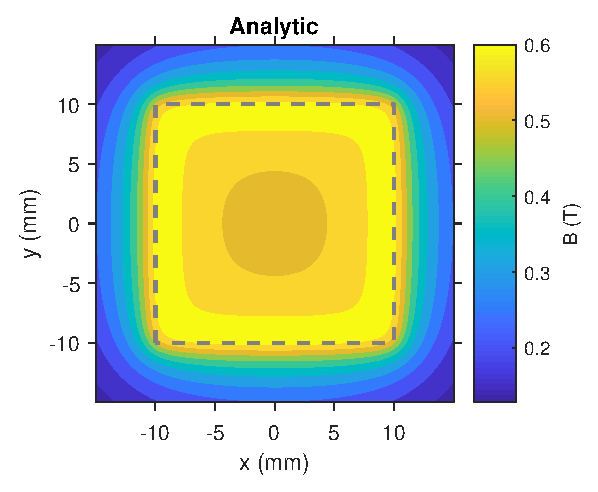
\includegraphics[width=\textwidth]{p2/p2FIG5a}
		\caption{}\label{fig:frustumfielda}\vspace{5mm}
	\end{subfigure}
	
	\begin{subfigure}{0.65\textwidth}
		\centering
		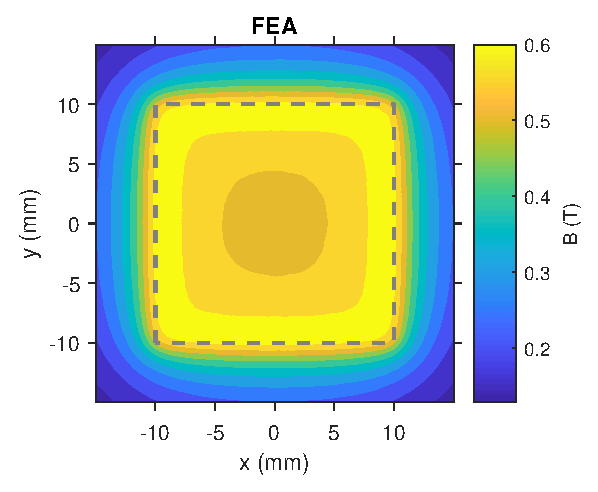
\includegraphics[width=\textwidth]{p2/p2FIG5b}
		\caption{}\label{fig:frustumfieldb}
	\end{subfigure}
	\caption{Magnetic field strength 1mm above the pyramid frustum magnet shown in Figure \ref{fig:p2frustum}, with the top surface of the magnet shown as a dashed line. The analytic calculation is shown in (\subref{fig:frustumfielda}), with the finite element calculation in (\subref{fig:frustumfieldb}). The maximum error between the two calculations is 0.7 percent, showing strong agreement.}
	\label{fig:p2frustumfield}
\end{figure}

\subsection{Cylindrical magnet}\label{sec:p2cylindricalmagnet}
\begin{figure}
	\centering
	\def\lim{13}

\tdplotsetmaincoords{70}{0}
\begin{tikzpicture}[scale=0.14,tdplot_main_coords]

% Draw cylinder
\draw (-10,0,-20) arc[radius = 10, start angle = -180, end angle = 0];
\draw (0,0,0) circle [radius = 10];
\draw (-10,0,0) -- (-10,0,-20);
\draw (10,0,0) -- (10,0,-20);

% Axes:
\draw[->] (0,0,0) -- (\lim,0,0);
\draw[->] (0,0,0) -- (0,0,\lim);
\node(xaxis) at (\lim+2,0,0) {\(x\)};
\node(zaxis) at (0,0,\lim+2) {\(z\)};

% Dimensions:
\draw[<->] (0,0,-27) -- (10,0,-27);
\node(radius) at (5,0,-30) {10mm};
\draw[<->] (-15,0,-20) -- (-15,0,0);
\node(height) at (-20,0,-10) {20mm};

\end{tikzpicture}
	\caption{A cylindrical permanent magnet. It has a radius of 10\si{\milli\metre}, a height of 20\si{\milli\metre}, and a magnetisation of \num{1.035e6}\si{\ampere\per\metre} (1.3\si{\tesla}) in the positive \(z\) direction.}
	\label{fig:p2cylinder}
\end{figure}
To further validate the analytic algorithm, a cylindrical geometry was examined, as shown in Figure \ref{fig:p2cylinder}. This magnet is an axially-magnetised cylindrical magnet with a radius of 10\si{\milli\metre}, a height of 20\si{\milli\metre}, and a magnetisation strength of \num{1.035e6}\si{\ampere\per\metre} (1.3\si{\tesla}). The magnetic field is again measured across a plane positioned \(z = 1\)\si{\milli\metre} above the top surface of the magnet using a \(301\times301\) grid of points on a 30\si{\milli\metre} \(\times\) 30\si{\milli\metre} region (0.1\si{\milli\metre} grid spacing using 90601 gridpoints).

Firstly, the exact magnetic field was calculated using the analytic equations published by \textcite{Caciagli2018}. Then, the geometry was input into Maxwell3D and a simulation carried out using approximately \num{9.6e5} tetrahedral elements (approximately \num{1.7e5} inside the magnet and \num{7.9e5} in the region outside the magnet). The cylinder was finally approximated as a polygonal prism, with the cross section being a 32-gon and an equivalent radius to maintain the same volume as the cylinder. Equation (\ref{eqn:p2fieldequation}) was applied to this polygonal prism to approximate the solution of a cylindrical magnet using a polyhedral magnet, and the results of all three calculations shown in Figure \ref{fig:p2cylinderfield}.

The maximum field strength was 0.571\si{\tesla} (this work), 0.573\si{\tesla} (FEA), and 0.571\si{\tesla} (exact \cite{Caciagli2018}). When compared to the exact result, the polyhedral approximation using this work gives a maximum error of less than 0.1 percent. When compared to the FEA simulation, the polyhedral approximation gave a maximum error of 0.8 percent. This implies the polyhedron is able to accurately approximate a cylindrical permanent magnet. More detailed results are given in \ref{sec:p2detailedResults}.

Again, it is difficult to compare the computation time of the algorithm presented in this paper and FEA simulations. The simulations took approximately 38 minutes to calculate the field at any number of points, whereas the algorithm here took approximately 0.9 seconds to calculate the field at 90601 points.

Additionally, this calculation was validated using previous published and validated work by the current authors \cite{OConnell2020}. The error was within numerical noise, but the algorithm presented in this paper calculated the field orders of magnitude faster.
\begin{figure}
	% Colour should be used for this figure
	\centering
	\begin{subfigure}{0.47\textwidth}
		\centering
		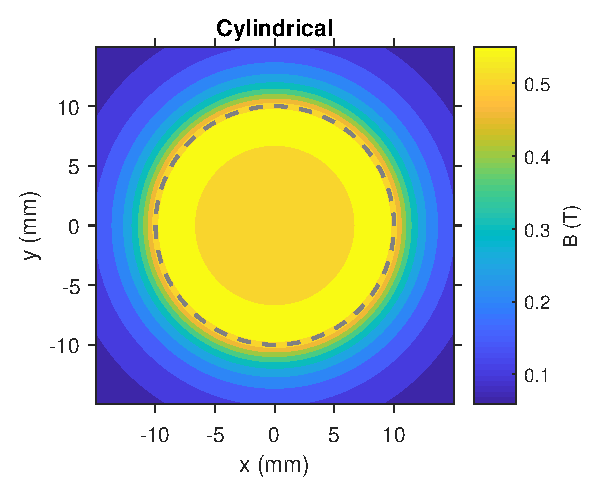
\includegraphics[width=\textwidth]{p2/p2FIG7a}
		\caption{}\label{fig:p2cylinderfielda}
	\end{subfigure}
	~
	\begin{subfigure}{0.47\textwidth}
		\centering
		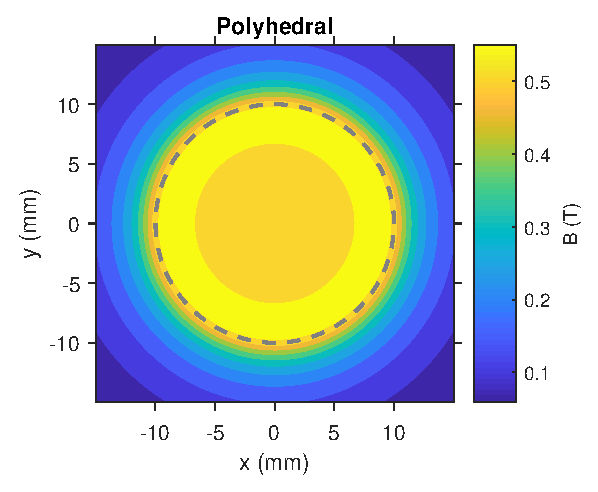
\includegraphics[width=\textwidth]{p2/p2FIG7b}
		\caption{}\label{fig:p2cylinderfieldb}
	\end{subfigure}
	
	\vfill
	\begin{subfigure}{0.47\textwidth}
		\centering
		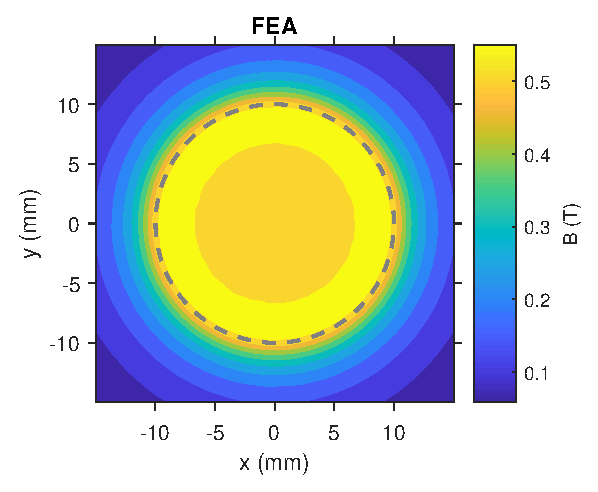
\includegraphics[width=\textwidth]{p2/p2FIG7c}
		\caption{}\label{fig:p2cylinderfieldc}
	\end{subfigure}
	\caption{Magnetic field strength 1\si{\milli\metre} above the cylindrical magnet shown in Figure \ref{fig:p2cylinder}, with the top surface of the magnet shown as a dashed line. The analytic cylindrical field \cite{Caciagli2018} is shown in (\subref{fig:p2cylinderfielda}), the polyhedral field shown in (\subref{fig:p2cylinderfieldb}), and the finite element calculation in (\subref{fig:p2cylinderfieldc}). The maximum percentage error between the exact cylinder field \cite{Caciagli2018} and polyhedral field was less than 0.1 percent, indicating it is an accurate approximation to a cylindrical magnet.}
	\label{fig:p2cylinderfield}
\end{figure}

\subsection{Polyhedral approximation of curved surfaces}
In the previous section, it was shown that an extruded 32-gon magnet is able to accurately approximate an axially-magnetised cylindrical magnet. This was validated using slow FEA simulations and the much faster analytic solution published by \textcite{Caciagli2018}. However, no analytic field solutions for general curved surfaces exist in literature, and FEA is slow and is impractical for real-time simulations. Instead, polyhedra can be used to approximate these surfaces for a fast-solving and accurate solution. To produce more accurate results, a polyhedron with a larger number of faces can be used; to achieve a faster calculation, a polyhedron with fewer faces can be used. This section shows an example of this tradeoff between accuracy and calculation time by approximating a cylindrical magnet with an extruded polygon with a varying number of sides, \(n\).

To quantify the error of the polyhedral approximation, the cylindrical magnet defined in Section \ref{sec:p2cylindricalmagnet} was considered. The magnetic field produced by this magnet was calculated using the equations published by \textcite{Caciagli2018} at a point 1\si{\milli\metre} above the central axis of the magnet, \(\mathbf{x} = \left[ 0, 0, 1\right]\)\si{\milli\metre}, and a point 1\si{\milli\metre} above the circumference of the top surface, \(\mathbf{x} = \left[ 10, 0, 1 \right]\)\si{\milli\metre}. The magnet was then approximated as a regular polygonal prism with a given number of sides \(n\), and the magnetic field calculated at the two aforementioned points. As the number of sides of the polygon \(n\) was increased, the error between the fields produced by cylindrical magnet and polyhedral magnet was calculated and recorded.

At the point \(\mathbf{x} = \left[ 0,0,1\right]\)\si{\milli\metre}, the exact magnetic field strength \cite{Caciagli2018} is 0.52\si{\tesla}. For a point along the axis of this magnet, the field can also be found using the difference between two cosines, giving the same result. The percentage error between this value and the magnetic field strength due to a polyhedral approximation was calculated for each \(n\) and is shown in Figure \ref{fig:p2polycylapproxa}. The polyhedral approximation is most impactful near the curved surface of the magnet, since this is where the geometry has been changed most significantly. Therefore, at the point \(\mathbf{x} = \left[ 0,0,1\right]\)\si{\milli\metre}, the polyhedral approximation is negligible and the error small since this point is far from the curved surface. The \(n = 32\) approximation from Section \ref{sec:p2cylindricalmagnet} takes approximately 28\si{\milli\second} to calculate the field and gives an error of \num{2.4e-5} percent. Alternatively, halving the number of sides (\(n = 16\)) takes approximately 17\si{\milli\second} to calculate the field while giving a larger error of \num{4.1e-4} percent.

At the point \(\mathbf{x} = \left[ 10,0,1\right]\)\si{\milli\metre}, the exact magnetic field strength \cite{Caciagli2018} is 0.53\si{\tesla}. The error between this field strength and the field strength due to the polyhedral approximation was again calculated and is shown in Figure \ref{fig:p2polycylapproxb}. This point is significantly closer to the curved surface of the magnet, and the error is therefore larger than at the point \(\left[ 0,0,1\right]\)\si{\milli\metre}. However, the error is still negligible for sufficiently large \(n\). The \(n = 32\) approximation from Section \ref{sec:p2cylindricalmagnet} takes approximately 29\si{\milli\second} to calculate the field and gives an error of \num{2.8e-2} percent. Alternatively, halving the number of sides (\(n = 16\)) takes approximately 16\si{\milli\second} to calculate the field while giving a larger error of \num{4.5e-1} percent.
\begin{figure}
	\centering
	\begin{subfigure}{0.6\textwidth}
		\centering
		\includegraphics[width=\textwidth]{p2/p2FIG8a}
		\caption{}\label{fig:p2polycylapproxa}
	\end{subfigure}
	
	\begin{subfigure}{0.6\textwidth}
		\centering
		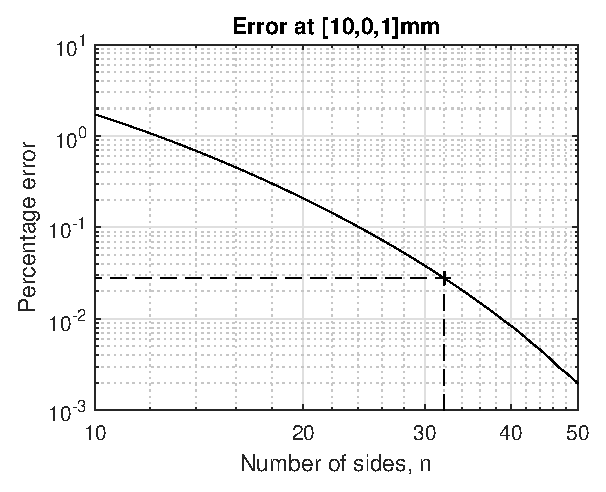
\includegraphics[width=\textwidth]{p2/p2FIG8b}
		\caption{}\label{fig:p2polycylapproxb}
	\end{subfigure}
	\caption{Error in the magnetic field strength produced by a polygonal prismatic magnet approximation of a cylindrical magnet as the number of sides of the polygon, \(n\), is increased. The \(n = 32\) approximation from Section \ref{sec:p2cylindricalmagnet} is highlighted. At the point \(\mathbf{x} = \left[0,0,1\right]\)\si{\milli\metre} (\subref{fig:p2polycylapproxa}), the magnetic field strength is 0.52\si{\tesla}, leading to an error of \num{2.4e-5} percent for a 32-gon approximation. At the point \(\mathbf{x} = \left[10,0,1\right]\)\si{\milli\metre} (\subref{fig:p2polycylapproxb}), the magnetic field strength is 0.53\si{\tesla}, leading to an error of \num{2.8e-2} percent for a 32-gon approximation.}
	\label{fig:p2polycylapprox}
\end{figure}

These results indicate that polyhedral permanent magnets can be used to approximate curved magnets and that a larger number of polygonal surfaces leads to a more accurate solution at the cost of a larger calculation time. Additionally, as the point \(\mathbf{x}\) approaches a curved magnet surface, a greater number of polyhedral facets are required for accurate field computations. This is particularly useful for magnet geometries with no analytic solution such as general curved surfaces. This approximation is considerably faster than FEA simulations, while maintaining high accuracy.
\section{Conclusion}\label{sec:p2conclusion}
This paper has outlined a new fully analytic and fast method for calculating the magnetic field produced by a polyhedral permanent magnet. The methodology was presented, outlining the process of decomposition and giving the solution to the charge model for a charged trapezium, leading to the total field produced by the polyhedral magnet. Singular regions were identified, and their solutions presented. This was followed by a validation section showing strong agreement between finite element simulations, literature, and the work detailed here. The magnetic field equations presented here are less complicated and more efficient than those in current literature since only two rotations are required per facet, independent of the number of magnetic field calculations.

The equations had high accuracy when compared to finite element simulations and literature using both a pyramid frustum magnet and a cylindrical magnet. The equations were validated against the finite element simulations and literature, giving a maximum error of less than 1 percent for both the frustum and cylindrical magnets.

It was shown that curved surfaces can be approximated as polyhedral surfaces and this methodology applied. A cylindrical magnet was approximated as a polygonal prism with an arbitrary number of sides. It was shown that both the accuracy and computation time increased with the number of sides. For the case considered, it was shown that the error was less than 0.1 percent using a 32-gon prismatic magnet, taking less than 30\si{\milli\second} to compute the field.

Currently, finite element simulations are usually used to analyse complicated magnetic systems. However, this is slow and optimisation of magnet shape or topology can take a considerable amount of time. The methodology presented here can be used to analyse these complicated magnetic systems far more quickly than finite element simulations. Furthermore, due to the simplicity and speed of calculation, it can be used for approximation of complicated magnet shapes, real-time simulations, or optimisation of magnet shape and topology to quickly arrive at a desired magnetic field.
\begin{subappendices}
\addcontentsline{toc}{section}{\protect\numberline{}Appendices}
\addtocontents{toc}{\protect\setcounter{tocdepth}{-1}}
\renewcommand{\thesection}{Appendix \arabic{chapter}.\Alph{section}}
\section{Derivation of \texorpdfstring{\(R\)}{R}}\label{sec:p2Rderivation}
The derivation of the rotation matrix \(R\) begins by defining a coordinate system on an arbitrary plane containing the polygonal surface \(S_{\!i}\). Let \(\left[ \hat{\mathbf{x}}, \hat{\mathbf{y}}, \hat{\mathbf{z}}\right]\) be the global coordinate system and let \(\hat{\mathbf{n}} = \left[ n_x, n_y, n_z\right]\) be the outward-facing unit normal vector of \(S_{\!i}\). We want to rotate this normal vector using the rotation matrix \(R\) such that \(\hat{\mathbf{n}} R = \hat{\mathbf{z}}\).

To do this, a coordinate system \(\left[ \hat{\mathbf{x}}', \hat{\mathbf{y}}', \hat{\mathbf{z}}' \right]\) is defined on the arbitrary plane such that \( \hat{\mathbf{n}} = \hat{\mathbf{z}}'\). To rotate \(\left[ \hat{\mathbf{x}}', \hat{\mathbf{y}}', \hat{\mathbf{z}}' \right]\) to \(\left[ \hat{\mathbf{x}}, \hat{\mathbf{y}}, \hat{\mathbf{z}}\right]\), a rotation matrix given by

\begin{equation}
R = \begin{bmatrix}
\hat{\mathbf{x}}'^{\textsf{T}} & \hat{\mathbf{y}}'^{\textsf{T}} & \hat{\mathbf{z}}'^{\textsf{T}}
\end{bmatrix}
\end{equation}

\noindent can be used.

Now, we have already defined

\begin{equation}
\hat{\mathbf{z}}' = \hat{\mathbf{n}} = \left[ n_x, n_y, n_z \right] \text{,}
\end{equation}

\noindent and \(\hat{\mathbf{x}}'\) and \(\hat{\mathbf{y}}'\) can be defined arbitrarily, provided \(\hat{\mathbf{x}}'\), \(\hat{\mathbf{y}}'\), and \(\hat{\mathbf{z}}'\) are mutually orthogonal unit vectors.

Without loss of generality, define \(\hat{\mathbf{y}}' = \left[ 0, y_2, y_3\right]\). We know that the dot product of \(\hat{\mathbf{y}}'\) and \(\hat{\mathbf{z}}'\) will be 0, since they are orthogonal. Therefore,

\begin{equation}\label{eqn:p2y2y3}
\hat{\mathbf{z}}' \cdot \hat{\mathbf{y}}' = 0 + n_y y_2 + n_z y_3 = 0 \implies y_2 = -\frac{n_z}{n_y} y_3 \text{.}
\end{equation}

\noindent We also know that \(\hat{\mathbf{y}}'\) is a unit vector, so

\begin{equation}\label{eqn:p2y2y32}
\left|\hat{\mathbf{y}}'\right| = \sqrt{y_2^2 + y_3^2} = \sqrt{\frac{n_z^2}{n_y^2} y_3^2 + y_3^2} = 1 \text{.}
\end{equation}

\noindent Solving Equations (\ref{eqn:p2y2y3}) and (\ref{eqn:p2y2y32}) gives

\begin{align}
y_2 &= \mp \frac{n_z}{\sqrt{n_y^2+n_z^2}} \\
y_3 &= \pm \frac{n_y}{\sqrt{n_y^2+n_z^2}} \text{.}
\end{align}

\noindent Taking the positive square root for \(y_2\) leads to

\begin{equation}
\hat{\mathbf{y}}' = \left[ 0, \frac{n_z}{\sqrt{n_y^2+n_z^2}}, -\frac{n_y}{\sqrt{n_y^2+n_z^2}} \right] \text{.}
\end{equation}

\noindent Finally, \(\hat{\mathbf{x}}'\) is simply given by \(\hat{\mathbf{x}}' = \hat{\mathbf{y}}' \times \hat{\mathbf{z}}'\). Therefore,

\begin{equation}
\hat{\mathbf{x}}' = \left[ \sqrt{n_y^2+n_z^2}, -\frac{n_xn_y}{\sqrt{n_y^2+n_z^2}}, -\frac{n_xn_z}{\sqrt{n_y^2+n_z^2}} \right] \text{.}
\end{equation}

\noindent Combining these gives the total rotation matrix

\begin{equation}
R = \begin{bmatrix}
\sqrt{n_y^2+n_z^2} & 0 & n_x \\
-\frac{n_xn_y}{\sqrt{n_y^2+n_z^2}} & \frac{n_z}{\sqrt{n_y^2+n_z^2}} & n_y \\
-\frac{n_xn_z}{\sqrt{n_y^2+n_z^2}} & -\frac{n_y}{\sqrt{n_y^2+n_z^2}} & n_z \end{bmatrix} \text{.}
\end{equation}

\subsection*{Solving \texorpdfstring{\(R\) for \(n_y = n_z = 0\)}{R for ny = nz = 0}}

If \(n_y = n_z = 0\) (and consequently \(n_x = \pm1\)), then \(R\) is undefined due to division by zero. Instead, let \(n_y = 0\) and take the limit as \(n_z \to 0^+\). Letting \(n_y = 0\) leads to \(\sqrt{n_y^2+n_z^2} = \left|n_z\right|\). Substituting \(n_y = 0\) into \(R\) and taking the limit of \(R\) as \(n_z \to 0^+\) gives

\begin{equation}
\lim_{n_z \to 0^+} R = \lim_{n_z \to 0^+} \begin{bmatrix}
\left|n_z\right| & 0 & 1 \\
0 & \sgn n_z & 0 \\
- \sgn n_z & 0 & 0
\end{bmatrix} \text{,}
\end{equation}

\noindent where \( \sgn n_z \) is the sign of \(n_z\). \(\lim_{n_z \to 0^+} \sgn n_z\) is unity, and \(\lim_{n_z \to 0^+} \left|n_z\right|\) is zero. Therefore,

\begin{equation}
\lim_{n_z \to 0^+} R = \begin{bmatrix}
0 & 0 & 1 \\
0 & 1 & 0 \\
-1 & 0 & 0
\end{bmatrix} \text{.}
\end{equation}
\section{Number of trapezia on a polyhedral surface}\label{sec:p2numtrap}
Let \(S\) be a polyhedron composed of \(F\) polygonal surfaces \(S_{\!i}\), and let \(n_i\) be the number of edges of the polygon \(S_{\!i}\).

Consider one surface \(S_{\!i}\) (with \(n_i\) edges). Draw parallel lines across the surface of \(S_{\!i}\) passing through each vertex, creating up to \(n_i-1\) trapezia, \(T_{\!j}\), as shown in Figure \ref{fig:p2polyhedrondecompositionb}. Repeat for all surfaces \(S_{\!i}\). The maximum total number of trapezia on the surface of the polyhedron \(S\) is then

\begin{align*}
N_{\text{trapezia}} &= \sum_{i=1}^F \left( n_i - 1\right) \\
&= \left( \sum_{i=1}^F n_i\right) - F \text{.}
\end{align*}

Now, the summation term is counting each edge of each face \(S_{\!i}\). However, since each edge is shared between two faces, the summation term counts each edge twice. Therefore,

\begin{align*}
\sum_{i=1}^F n_i = 2E \text{,}
\end{align*}

\noindent where \(E\) is the number of edges of the polyhedron. Hence,

\begin{align*}
N_{\text{trapezia}} = 2E - F \text{.}
\end{align*}
\section{Detailed validation results}\label{sec:p2detailedResults}
This section includes more detailed information from Section \ref{sec:p2validation}, where the algorithm presented in this paper was validated using finite element simulations (FEA) and literature. The calculation time of each method and the error associated with each comparison is given.

\subsection*{Pyramid frustum magnet}

For this comparison, the field was calculated across a 301\(\times\)301 grid across a 30mm\(\times\)30mm region. The maximum field strength and RMS field strength for both analytical and FEA methods are given by

\begin{equation}\label{eqn:p2bmax}
	B_{\text{max}} = \text{max}\left(\left|\mathbf{B}_i\right|\right) \text{,}
\end{equation}

\begin{equation}\label{eqn:p2brms}
	B_{\text{RMS}} = \sqrt{\frac{1}{n} \sum_{i=1}^{n} \left| \mathbf{B}_i \right| ^2} \text{,}
\end{equation}

\noindent where \(n\) is the number of points at which the field is calculated and \(\mathbf{B}_i\) is the magnetic field at the \(i\)th point. The error between FEA and analytic evaluations is given by

\begin{equation}
\varepsilon_i = \Big|\big|\mathbf{B}_{\text{analytic,}i}\big|-\big|\mathbf{B}_{\text{FEA,}i}\big|\Big| \text{,}
\end{equation}

\noindent with the maximum and RMS error are defined as

\begin{equation}\label{eqn:p2errmax}
	\varepsilon_{\text{max}} = \text{max}\left(\varepsilon_i\right) \text{,}
\end{equation}

\begin{equation}\label{eqn:p2errrms}
	\varepsilon_{\text{RMS}} = \sqrt{\frac{1}{n} \sum_{i = 1}^n \varepsilon_i^2} \text{.}
\end{equation}

\noindent The percentage errors were also calculated by dividing the error at each point by the analytic magnetic field strength at that point,

\begin{equation}\label{eqn:p2errpc}
	\varepsilon_{\text{\%,}i} = \frac{\varepsilon_i}{\left|\mathbf{B}_{\text{analytic,}i}\right|} \times 100\% \text{.}
\end{equation}

\noindent The maximum and RMS percentage errors \(\varepsilon_{\text{\%,max}}\) and \(\varepsilon_{\text{\%,RMS}}\) were also calculated using equations similar to Equations (\ref{eqn:p2errmax}) and (\ref{eqn:p2errrms}). Results are shown in Table \ref{tab:p2frustumstats}. These results indicate strong agreement between the analytic methodology proposed in this paper and FEA simulations, with a maximum error less than 1 percent, indicating the analytic methodology is providing correct field computations.

\begin{table}
	\centering
	\caption{Results from the frustum magnet field calculation. The analytic calculation and FEA simulation produce similar results, with a maximum error of less than 1 percent between the two. The time taken to evaluate the analytic field is 0.3144\si{\second} for 90601 field points (averaging 3.470\si{\micro\second} per point).}
	\label{tab:p2frustumstats}
	\begin{tabular}{l | c c}
		& Analytic & FEA \\
		\hline
		\rule{0pt}{2.5ex}Time\textsubscript{total} (\si{\second}) & \num{0.3144} & 2462 \\
		\(B_{\text{max}}\) (\si{\tesla}) & 0.6332 & 0.6362 \\
		\(B_{\text{RMS}}\) (\si{\tesla}) & 0.4744 & 0.4743 \\
		\(\varepsilon_{\text{max}}\) (\si{\tesla}) &  & \num{4.042e-3} \\
		\(\varepsilon_{\text{RMS}}\) (\si{\tesla}) &  & \num{5.590e-4} \\
		\(\varepsilon_{\text{\%,max}}\) (\%) & & 0.7185 \\
		\(\varepsilon_{\text{\%,RMS}}\) (\%) & & 0.1316 \\
		\hline
	\end{tabular}
\end{table}

\subsection*{Cylindrical magnet}
The maximum and RMS field strengths were defined according to Equations (\ref{eqn:p2bmax}) and (\ref{eqn:p2brms}), and the polyhedral error and FEA error were defined as
\begin{equation}
	\varepsilon_{\text{polyhedron}} = \Big|\big|\mathbf{B}_{\text{cylinder,}i}\big| - \big|\mathbf{B}_{\text{polyhedron,}i}\big|\Big| \text{,}
\end{equation}
\begin{equation}
	\varepsilon_{\text{FEA}} = \Big|\big|\mathbf{B}_{\text{cylinder,}i}\big| - \big|\mathbf{B}_{\text{FEA,}i}\big|\Big| \text{,}
\end{equation}
\noindent where \(\mathbf{B}_{\text{cylinder}}\) is the exact magnetic field \cite{Caciagli2018}. The maximum and RMS errors were defined according to Equations (\ref{eqn:p2errmax}) and (\ref{eqn:p2errrms}), with the percentage errors being defined as
\begin{equation}
	\varepsilon_{\text{\%,}i} = \frac{\varepsilon_i}{\left|\mathbf{B}_{\text{cylinder,}i}\right|}\times100\% \text{.}
\end{equation}
\noindent The maximum and RMS percentage errors \(\varepsilon_{\text{\%,max}}\) and \(\varepsilon_{\text{\%,RMS}}\) were also calculated using equations similar to Equations (\ref{eqn:p2errmax}) and (\ref{eqn:p2errrms}). Results are shown in Table \ref{tab:p2cylinderstats}. Even though the cylinder was approximated as a polyhedron, the errors between the cylindrical field results, polyhedral field results, and FEA results are small. The FEA results had a maximum percentage error less than 1 percent when compared to the cylindrical calculation, whereas the polyhedral approximation had a maximum error less than 0.05 percent when compared to the analytic cylindrical calculation \cite{Caciagli2018}. This indicates that even with a polyhedral approximation of a cylinder, the analytic methodology proposed in this paper can give more accurate results than FEA. Additionally, the polyhedral approximation was considerably faster to evaluate than the FEA simulations. Furthermore, these results suggest that polyhedral approximations can provide accurate field computations for curved surfaces.
\begin{table}
	\centering
	\caption{Results from the cylindrical magnet field calculation. The polyhedral field and FEA field were compared against the analytic cylindrical field \cite{Caciagli2018}. The FEA results had an error less than 1 percent, whereas the polyhedral results had an error less than 0.05 percent. The total time taken to evaluate the magnetic field at 90601 points was 0.1304\si{\second} (averaging 1.439\si{\micro\second} per point) for the cylindrical calculation and 0.8668\si{\second} (averaging 9.567\si{\micro\second} per point) for the polyhedral calculation.}
	\label{tab:p2cylinderstats}
	\begin{tabular}{l | c c c}
		& Cylinder \cite{Caciagli2018} & Polyhedron & FEA \\
		\hline
		\rule{0pt}{2.5ex}Time\textsubscript{total} (\si{\second}) & 0.1304 & 0.8668 & 2258 \\
		\(B_{\text{max}}\) (\si{\tesla}) & 0.5710 & 0.5710 & 0.5731 \\
		\(B_{\text{RMS}}\) (\si{\tesla}) & 0.3815 & 0.3815 & 0.3814 \\
		\(\varepsilon_{\text{max}}\) (\si{\tesla}) & & \num{2.139e-4} & \num{3.337e-3} \\
		\(\varepsilon_{\text{RMS}}\) (\si{\tesla}) & & \num{3.534e-5} & \num{4.898e-4} \\
		\(\varepsilon_{\text{\%,max}}\) (\%) & & \num{4.317e-2} & 0.8118 \\
		\(\varepsilon_{\text{\%,RMS}}\) (\%) & & \num{7.436e-3} & 0.1612 \\
		\hline
	\end{tabular}
\end{table}
\end{subappendices}
\clearpage
\section*{Author's remarks on Chapter \ref{chap:paper2}}
In many magnetostatic analyses, the magnetic field is computed at a large number of points in space. As such, it is necessary to use a method which scales well with the number of field points. Upon comparison of the methods detailed in Chapters \ref{chap:paper1} and \ref{chap:paper2}, it can be seen that although the field equations in the current chapter are more complicated, the relatively expensive geometric deconstruction process only occurs once. Thus, when the field is computed at few points, the method outlined in Chapter \ref{chap:paper1} is preferred due to the simplified field equations. In contrast, when the field is to be computed at many points, the method in the current chapter is greatly preferred due to the effective scaling as the number of points increases. Furthermore, while only fields were calculated in this chapter, the force and torque methodology from Chapter \ref{chap:paper1} may be applied, leading to fast force and torque calculations.
\addtocontents{toc}{\protect\setcounter{tocdepth}{2}}

\newpage
\section*{References}
\addcontentsline{toc}{section}{\protect\numberline{}References}
\printbibliography[heading=none]